\documentclass{article}
\usepackage{fancyhdr}
\usepackage{tabu}
\usepackage[top=1in, bottom=1in]{geometry}
\usepackage{multirow}
\usepackage{graphicx}
\usepackage{setspace}
\usepackage{parskip}
\usepackage{pdfpages}
\usepackage{varwidth}
\usepackage{tocloft}
\usepackage{setspace}
\setlength{\parindent}{15pt}

%\pagestyle{fancy}

\begin{document}
%USAFA DFEC Header
	\noindent \begin{tabu} to \textwidth{l X[c] r}
	\multirow{5}{*}{
\includegraphics[width=0.75in]{DOD.jpg}} & 
	\textbf{United States Air Force Academy} &  
	\multirow{5}{*}{
\includegraphics[width=0.75in]{DFEC}}\\
	& \textbf{Department of Electrical and Computer Engineering} & \\
	& \tiny{USAF ACADEMY, COLORADO}\\
	\\ \\ \\
	\end{tabu}
%Start text here

	\hfill18 Oct 2013
	\hspace{0pt} \\
	\hspace{0pt} \\
	\hspace{0pt} \\
%\noindent Captain Ryan Silva \\
%Assistant Professor \\
%Department of Electrical and Computer Engineering \\
%2354 Fairchild Dr Ste 2F46C \\
%USAF Academy, CO 80840 \\

\noindent Dear Selection Committee,


I am thrilled to share with you my application for the Dean's Oxford Program.
I hope to convey in the attached documents why I am the best candidate for this program, based
not only on my qualifications and unrivaled contributions to the Cadet Wing to date, but also
based on my potential to inspire the Cadet Wing in the future. 

My dream is to show cadets how, with basic undergraduate skills, they can influence the lives of
people around the world. While leading multi-disciplinary senior capstone teams, 
I have noticed that cadets sometimes struggle to see the relevance of their research and find
difficulty finding inspiration. I plan on providing this inspiration by bringing
Oxford-caliber research opportunities in biomedical engineering back to USAFA through a 
partnership with the Oxford Center for Affordable Healthcare Technology.

Thank you for taking the time to review my application for the Dean's Oxford Program. I am
excited by this opportunity and its potential to help the Cadet Wing, who, I believe, stand to 
be the real benefactors of this amazing program and what I have to offer through it.

%\vspace{10mm}
\hspace*{2.3in} \noindent Very Respectfully, \\
\hspace*{2.5in} 
\includegraphics[scale=.5]{silvasig}  \\
\hspace*{2.5in} RYAN J. SILVA, Capt, USAF \\
\hspace*{2.5in} Assistant Professor   \\
\hspace*{2.5in} Department of Electrical and Computer Engineering  \\
\hspace*{2.5in} United States Air Force Academy, CO \\ 
\hspace*{2.5in} Desk: 333-6973 Cell: 303-507-1840

\renewcommand\cfttoctitlefont{\small}
\renewcommand\cftsecfont{\small}
\renewcommand\cftsubsecfont{\small}
\renewcommand\cftsecpagefont{\small}
\renewcommand\cftsubsecpagefont{\small}
\renewcommand\cftsecafterpnum{\setstretch{0.1}}
\renewcommand\cftsubsecafterpnum{\setstretch{0.1}}
\renewcommand\contentsname{\bf Attachments}\tableofcontents

\newpage

\section*{Attachment 1 \newline Essay}
\addcontentsline{toc}{section}{Attachment 1 - Why Oxford?}
	\centerline{\LARGE{\textbf{Why Oxford?}}} \hspace{0pt} \\
	\centerline{\Large{Captain Ryan Silva}}
	\centerline{\large{Assistant Professor}}
	\centerline{\large{Department of Electrical and Computer Engineering}}
	\centerline{\large{United States Air Force Academy}} \hspace{0pt} \\
\indent My ultimate goal in pursuing the Oxford experience is to bring world-class
biomedical engineering research opportunities to USAFA. The core academic
strengths of Oxford's Center for Affordable Healthcare Technology (OxCAHT) and
the open-source nature of their research paired with Oxford's matchless
geopolitical landscape make the University of Oxford the only English-speaking
university in the world with whom my research aspirations can be accomplished.
I believe bringing these biomedical engineering research opportunities back
to USAFA, through a partnership with OxCAHT, will allow for generations of cadets
and faculty to draw from the deep well that is research in innovative medical technology.
I also believe that I am the perfect candidate to accomplish
this lofty objective.

As an award-winning project mentor for the senior capstone project
NeuMimic, funded through FalconWorks, I would bring OxCAHT valuable experience after leading a
successful multi-disciplinary, systems-level biomedical engineering research project. I would 
come armed with valuable leadership experience paired with technical expertise in signal 
processing and embedded systems, thereby establishing myself as an immediate contributor;
it is important to note that the director of OxCAHT, Dr. Gari Clifford, agrees
with my assessment. Dr. Clifford, after a \emph{very} thorough Skype interview,
offered me a place on his team; in fact, he already has a project in mind for me to work on. 
The project is outlined in a signed MFR that can be found in Attachment 1.1. 
Because of my engineering experience, Dr. Clifford has already scaled the project so that I may
complete it in three years. I am so excited at the prospect of pursuing this project 
because it feels as though this opportunity was tailored to suit my strengths and interests! 
 
Based on its potential contributions to human wellbeing, there are few fields
that offer more inspiring opportunities for research than biomedical engineering, especially the subject areas involving medical diagnostics.
Diagnostics is a very challenging discipline as it usually involves
prohibitively expensive and immobile equipment that regularly forces patients
to travel great distances at great cost in order to access care. These traits
currently inherent to medical diagnostics regularly exclude certain
populations from receiving proper
treatment. Affected populations can range from military members operating in an
expeditionary environment to inhabitants of rural communities, especially in the developing
world. My proposed research seeks to develop solutions to the critical need for
point-of-care devices that are cheap, power-efficient, reliable, and
transportable. The immediate impact of this research is clear: it will allow
individuals to access healthcare that otherwise would not be available. Oxford's
centuries-old geopolitical affiliations allow this type of research to progress 
at a pace unrivaled at any other university or center. This is proven by the
expectations of the program, which involve identifying a real-world diagnostic 
shortfall, creating a novel solution to fill the need and conducting
clinical trials, all within the standard three-year time frame necessary to 
complete the degree. There is simply no other place on earth where medical research of
this type can progress from idea to government-sponsored field tests within this relatively short
time frame. While it is important to emphasize that this is exciting research,
it is also important to highlight where USAFA cadets fit in.
 
OxCAHT follows a research model based on the mission of Engineering World
Health ``to inspire and mobilize the biomedical engineering community to improve
the quality of health care in resource-poor communities of the developing
world" (www.oxcaht.org) . The ``mobilization" aspect of the above mission
statement effectively created a desire within the biomedical engineering 
community to take the handcuffs off traditional academic research. This has
been accomplished by embracing an open-source paradigm for conducting research.
The result of this paradigm is the creation of a ``Wikipedia" for biomedical
engineering research called PhysioNet, which is an open-source repository of
academic endeavors to which anyone may contribute. This repository is
predominately comprised of computer source code and raw diagnostic data but
also contains hardware schematics, mechanical drawings and other documentation
of studies, technologies, and data contributing to the field of biomedical
engineering. The open-source nature of this research is particularly
interesting when incorporated with the research climate of USAFA.
 
I have already laid down the ground work for developing a research partnership 
between Oxford and USAFA based on open-source technology through PhysioNet. 
I have garnered approvals through Col Kraus, USAFA Office of Research, and the
USAFA Judge Advocate for the research partnership I am proposing (the
approvals can be found in Attachments 1.2 and 1.3
respectively). Essentially, I can bring Oxford-level research opportunities to USAFA
now, so that younger cadets can reap the benefits, but I cannot accomplish this without
the Dean's Oxford Scholarship and the experience that comes with it. With this first step,
I can help generations of cadets make tangible contributions to the health and wellbeing of humanity.
Currently, Dr. Clifford needs help designing and implementing embedded solutions
for a plethora of diagnostic shortfalls. His center does an amazing job
identifying diagnostic issues in the developing world and creating advanced algorithms that use
state-of-the-art machine learning and novel signal processing techniques to
properly analyze diagnostics data, but what he is missing is a team of
undergraduates willing to implement the OxCAHT solutions in hardware such that
they can be tested in the field. This is where USAFA cadets come in. My experience with 
NeuMimic demonstrates that USAFA cadets are capable of developing and implementing biomedical 
signal processing techniques because they are already doing it. My experience has also taught me that
cadets are excited by research in biomedical engineering because its relevance is clear and immediate:
their efforts will help people. I can only
imagine what USAFA cadets could accomplish if they could meet and work with
expert researchers at OxCAHT! Once a partnership is established between Oxford and USAFA,
cadets could expect to create hardware platforms that make OxCAHT's advanced processing techniques
work in real life. These devices could then be transferred back to Oxford, through Physionet,
where they will be tested and, quite possibly, administered to real patients by Oxford researchers.
This opportunity is unparalleled!

I want to state unequivocally that my assignment at USAFA has easily been the
most rewarding experience of my career. I am truly passionate about the USAFA
Mission and I believe there is no greater professional fulfillment than to see
the sheer magnitude of positive influence and inspiration an officer can have
in a cadet's life. I have found that this is accomplished through tireless
devotion in and out of the classroom. My first tour has taught me to appreciate
the immense responsibility associated with shaping and motivating America's
future leaders, and it would be a privilege and an honor to be trusted with
that responsibility again by selecting me to bring Oxford-caliber opportunities
back to USAFA as a senior military faculty member. My resume clearly illustrates that I have thrived during my time in DFEC as I
have won every award the department has to give as well as garnered national
level recognition as the Great Minds in STEM Most Promising Engineer of 2013,
but there is no formal record of the three accolades I hold most dear: I have been
afforded the opportunity to participate in the culmination of the USAFA Mission
through administering the Oath of Office thereby commissioning three cadets into
Active Duty. When considering who should administer the Oath, cadets are
instructed to select the officer whose inspiration had the greatest impact on
their development and whose leadership they would most like to emulate. It is
humbling to consider that these (now) Lieutenants in the classes of 2011, 2012
and 2013 selected me to be a part of the zenith of their USAFA careers and the
arbiter that bestows upon them the prize for which they have worked so hard.
Ultimately my personal commitment to the USAFA Mission has been recognized by
my fellow faculty and endorsed by cadets, whose interests USAFA exists to
serve. By selecting me for the Dean's Oxford Scholarship, you afford me the opportunity
to further serve USAFA and its future officers.

%\vspace{10mm}
%\hspace*{2.3in} \noindent Very Respectfully, \\
%\hspace*{2.5in} 
\includegraphics[scale=.5]{silvasig}  \\
%\hspace*{2.5in} RYAN J. SILVA, Capt, USAF \\
%\hspace*{2.5in} Assistant Professor   \\
%\hspace*{2.5in} Department of Electrical and Computer Engineering  \\
%\hspace*{2.5in} United States Air Force Academy, CO  \\

%Original TOC
%\newpage
%\renewcommand\contentsname{Attachments}\tableofcontents

\newpage
\section*{Attachment 1.1 \newline Approved Oxford Research Proposal}
\addcontentsline{toc}{subsection}{Attachment 1.1 - Approved Oxford Research
Proposal}
\label{sec:prop}
\centering
\vspace{-5mm}
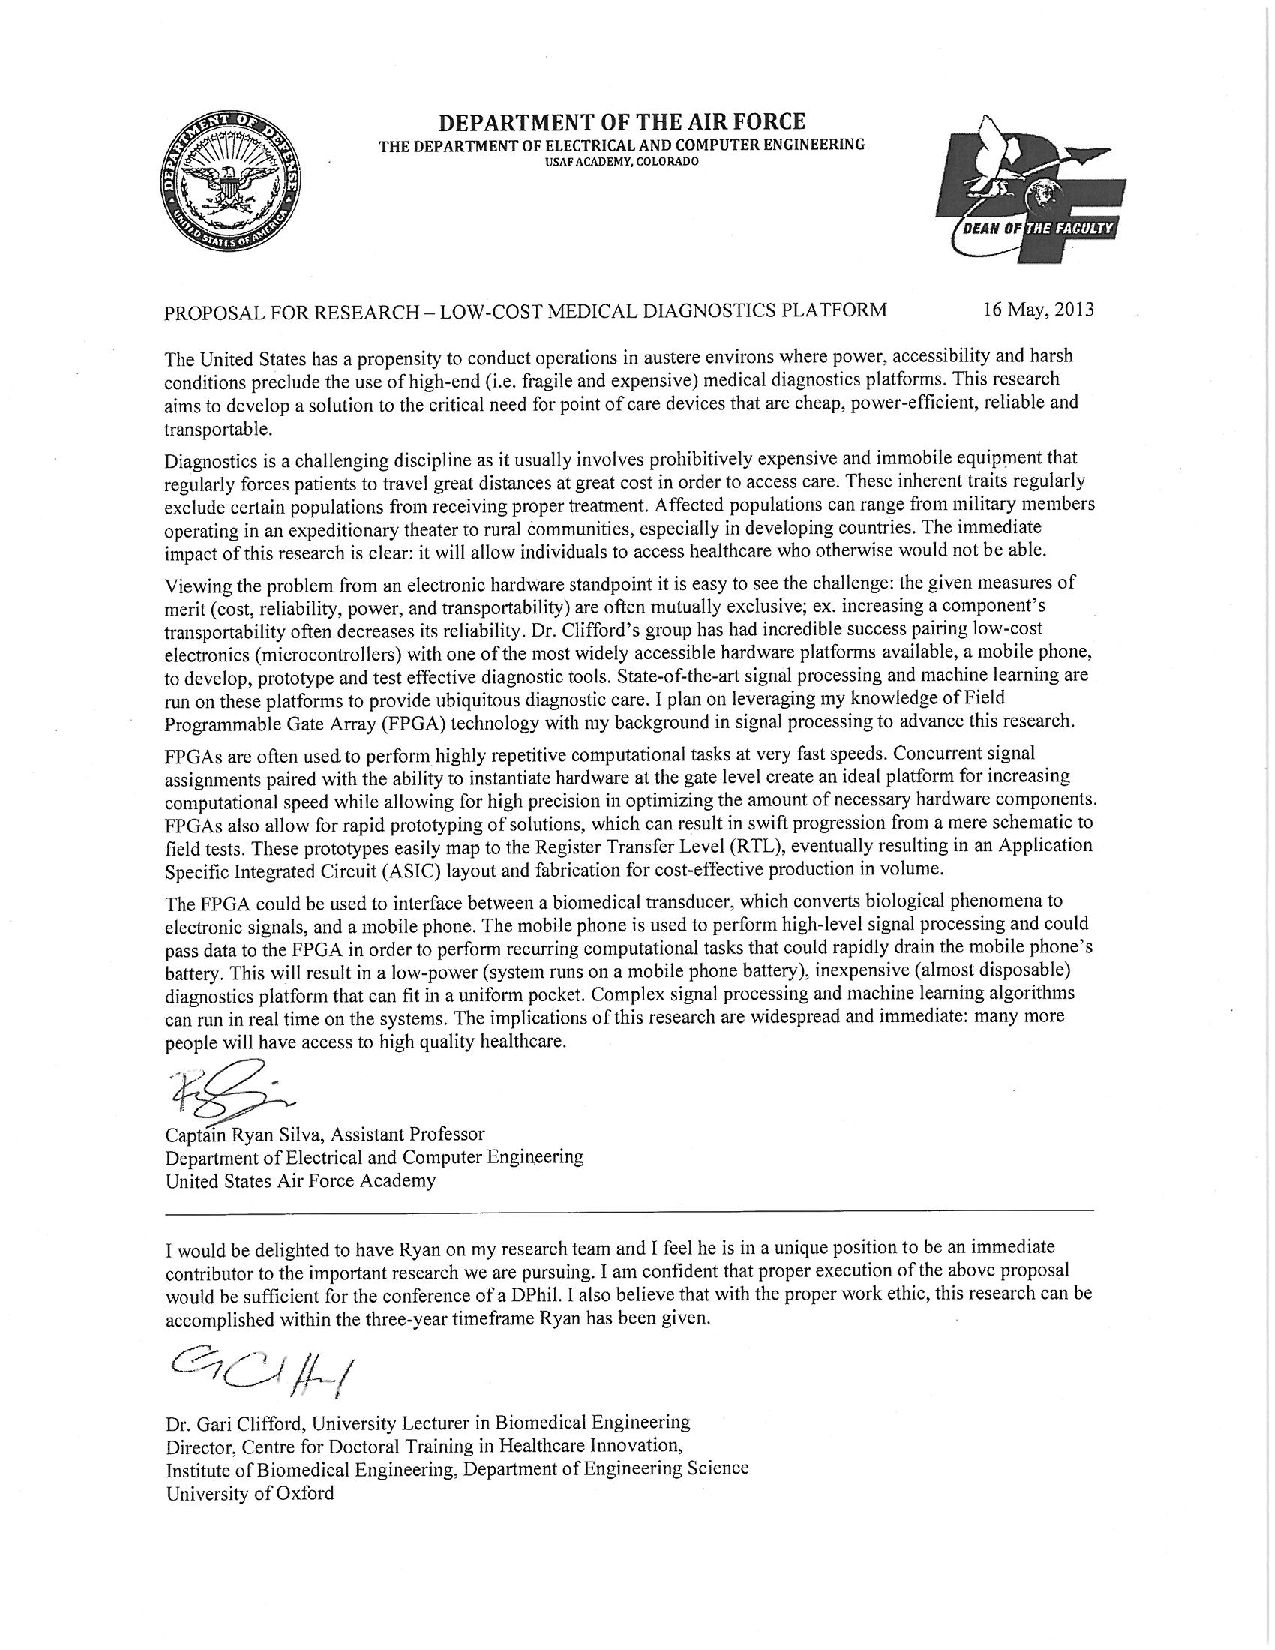
\includegraphics[scale=.85,clip=true,trim=1in .5in 1cm 0.4in]{MFR_ProposalforResearch_SilvaSIGNED.pdf}

\newpage
\section*{\raggedright Attachment 1.2 \newline DF Office of Research Approval to Conduct Research}
\addcontentsline{toc}{subsection}{Attachment 1.2 - DF Office of Research Approval to
Conduct Research}
\label{sec:DFER}
\centering
\vspace{-1cm}
\hspace*{-1.5cm}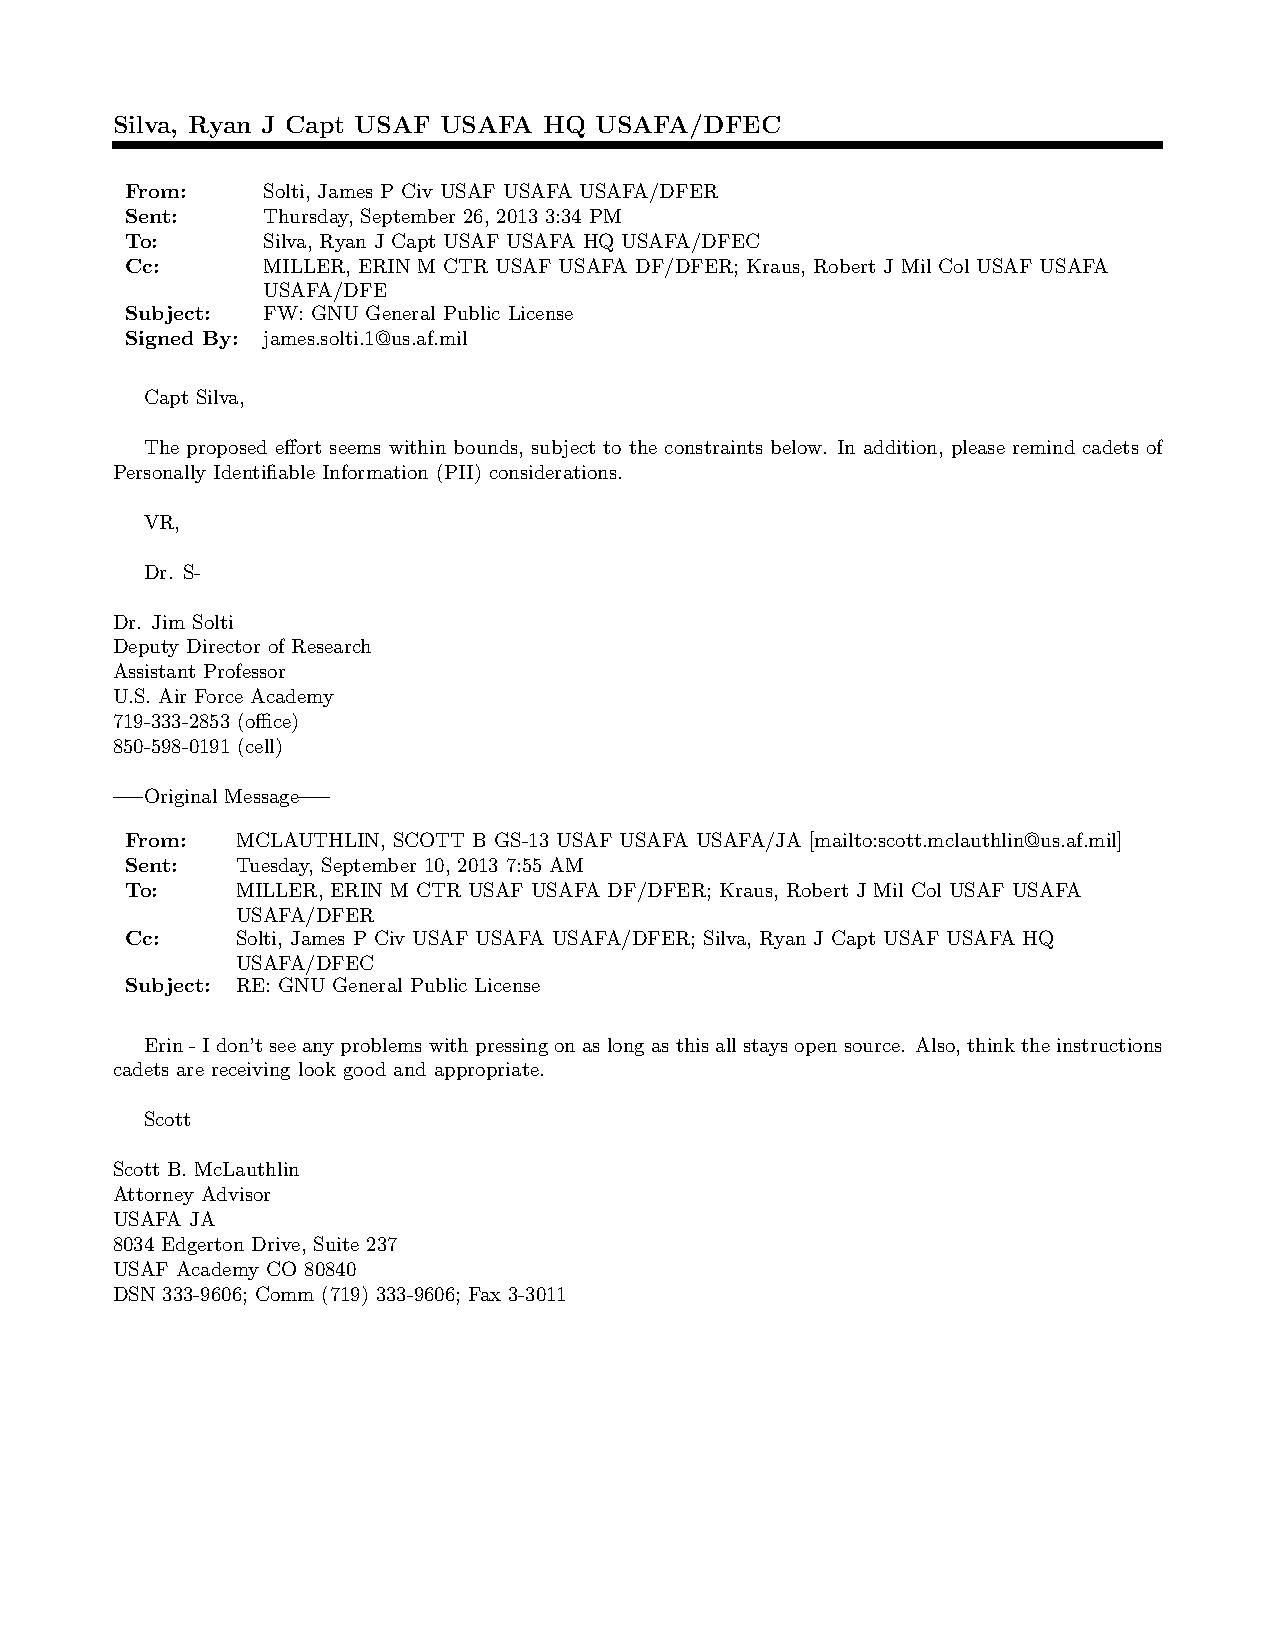
\includegraphics[scale=.85]{DFER_email.pdf}
\includepdf[pages=2-3,scale=0.85,offset=-0 -05,pagecommand={}]{DFER_email.pdf}
\newpage
\section*{\raggedright Attachment 1.3 \newline USAFA Judge Advocate Approval to Conduct Research}
\addcontentsline{toc}{subsection}{Attachment 1.3 - USAFA Judge Advocate Approval to
Conduct Research}
\label{sec:JA}
\centering
\vspace{-1cm}
\hspace*{-1.5cm}
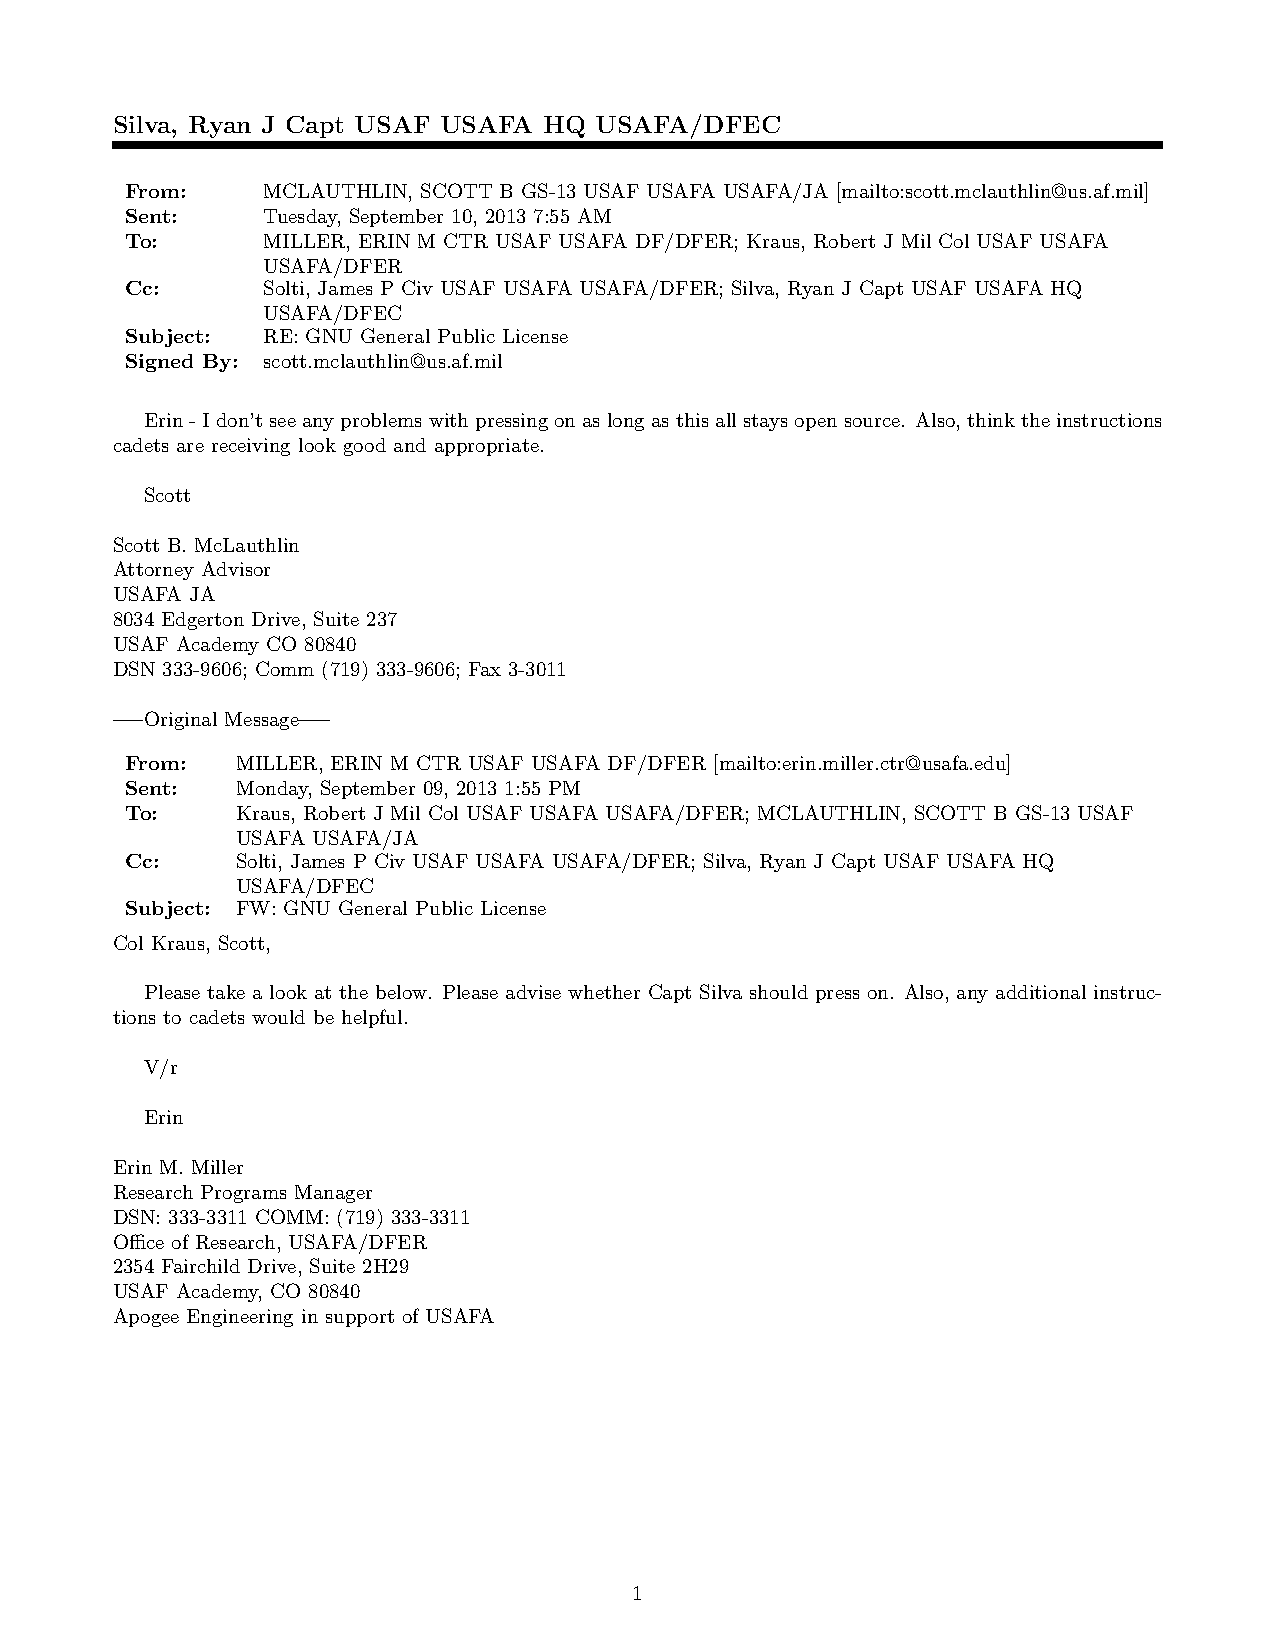
\includegraphics[scale=.85]{email.pdf}
\includepdf[pages=2,scale=0.85,offset=-0 -05,pagecommand={}]{email.pdf}

\newpage
\section*{\raggedright Attachment 2 \newline Ryan Silva Curriculum Vitae}
\addcontentsline{toc}{section}{Attachment 2 - Ryan Silva Curriculum Vitae}
\label{sec:CV}
\centering
\vspace{-1cm}
\hspace*{-1.5cm}
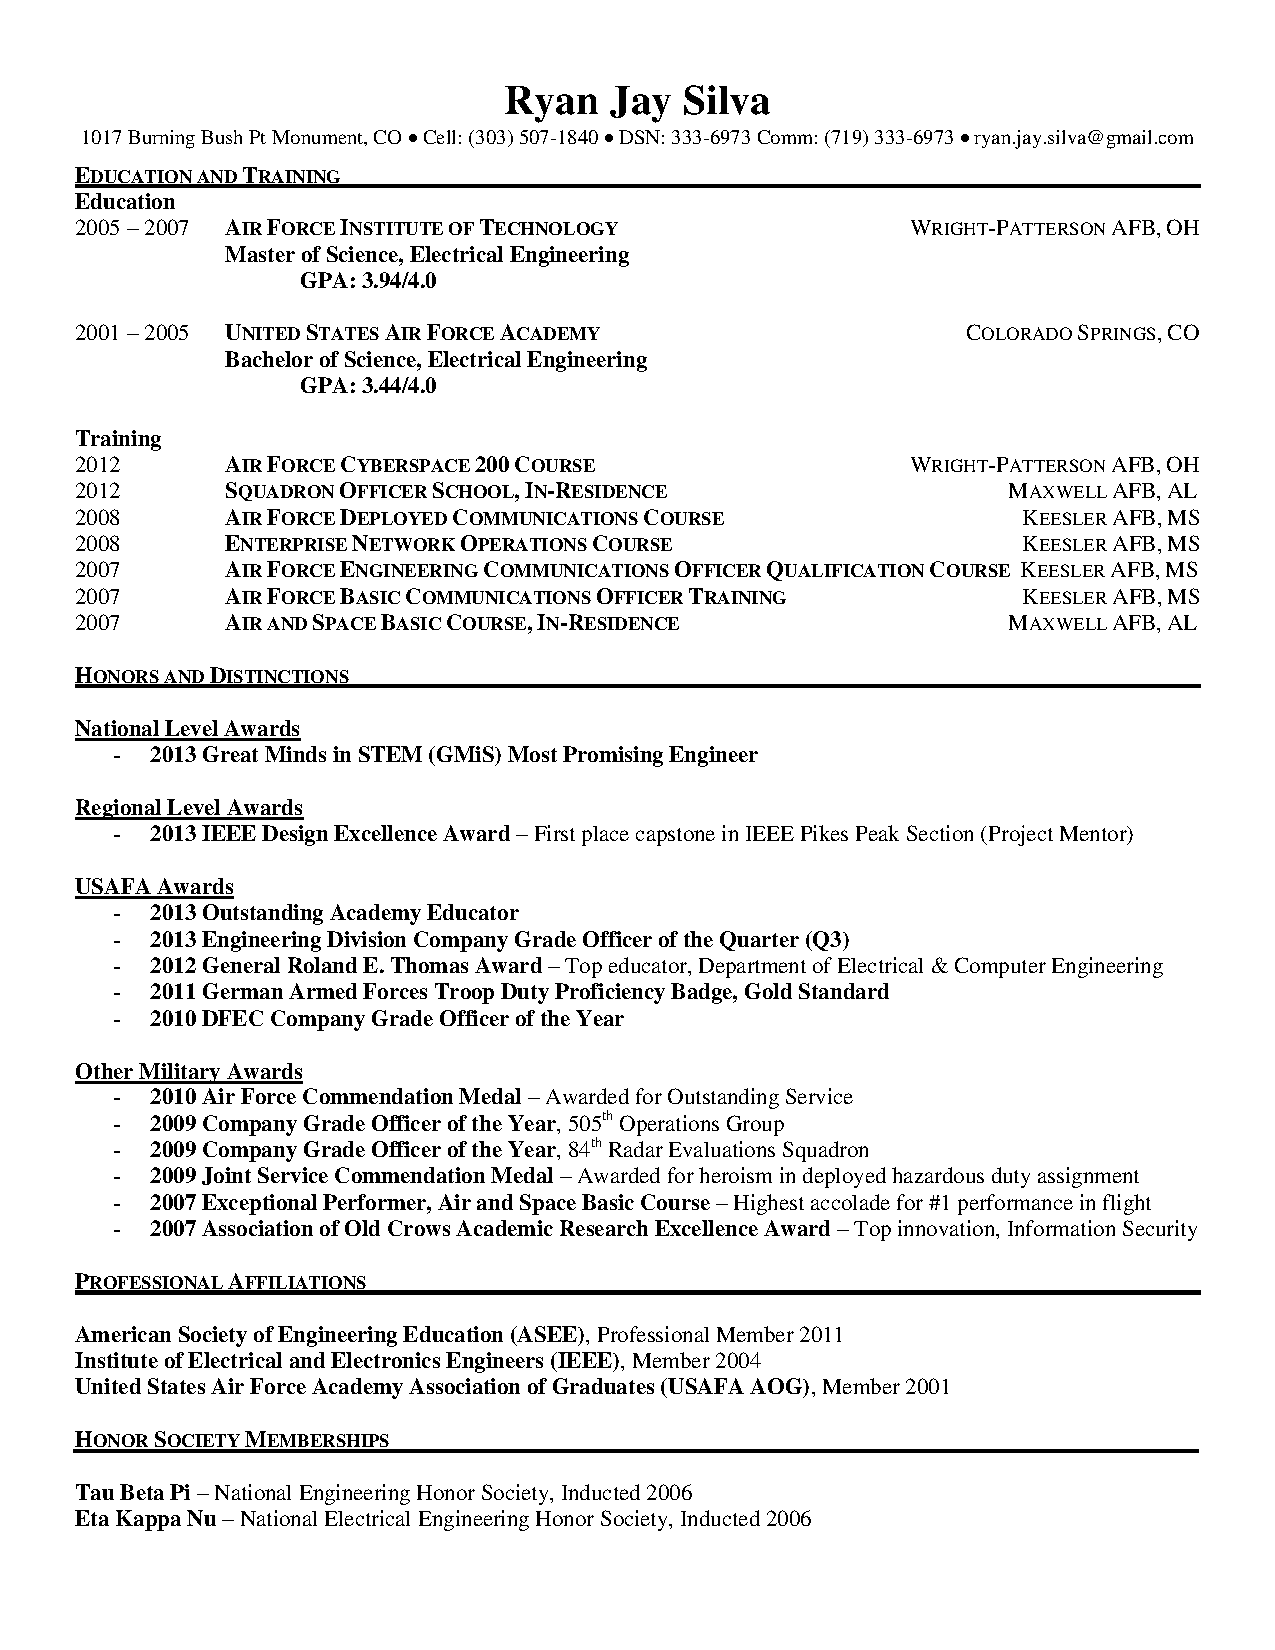
\includegraphics[scale=.85]{Oxford_CV_Silva.pdf}
\includepdf[pages=2-4,scale=0.85,offset=-0 -05,pagecommand={}]{Oxford_CV_Silva.pdf}

\newpage
%\section*{\raggedright Attachment 5 \newline DFEC Department Head Endorsement}
%\addcontentsline{toc}{section}{Attachment 5 - DFEC Department Head Endorsement}
%\label{sec:DFECHead}
\section*{\raggedright Attachment 3 \newline DFEC Department Head Endorsement}
\addcontentsline{toc}{section}{Attachment 3 - DFEC Department Head Endorsement}
\label{sec:DFECHead}
\centering
%\vspace{-1cm}
%\hspace*{-2.2cm}
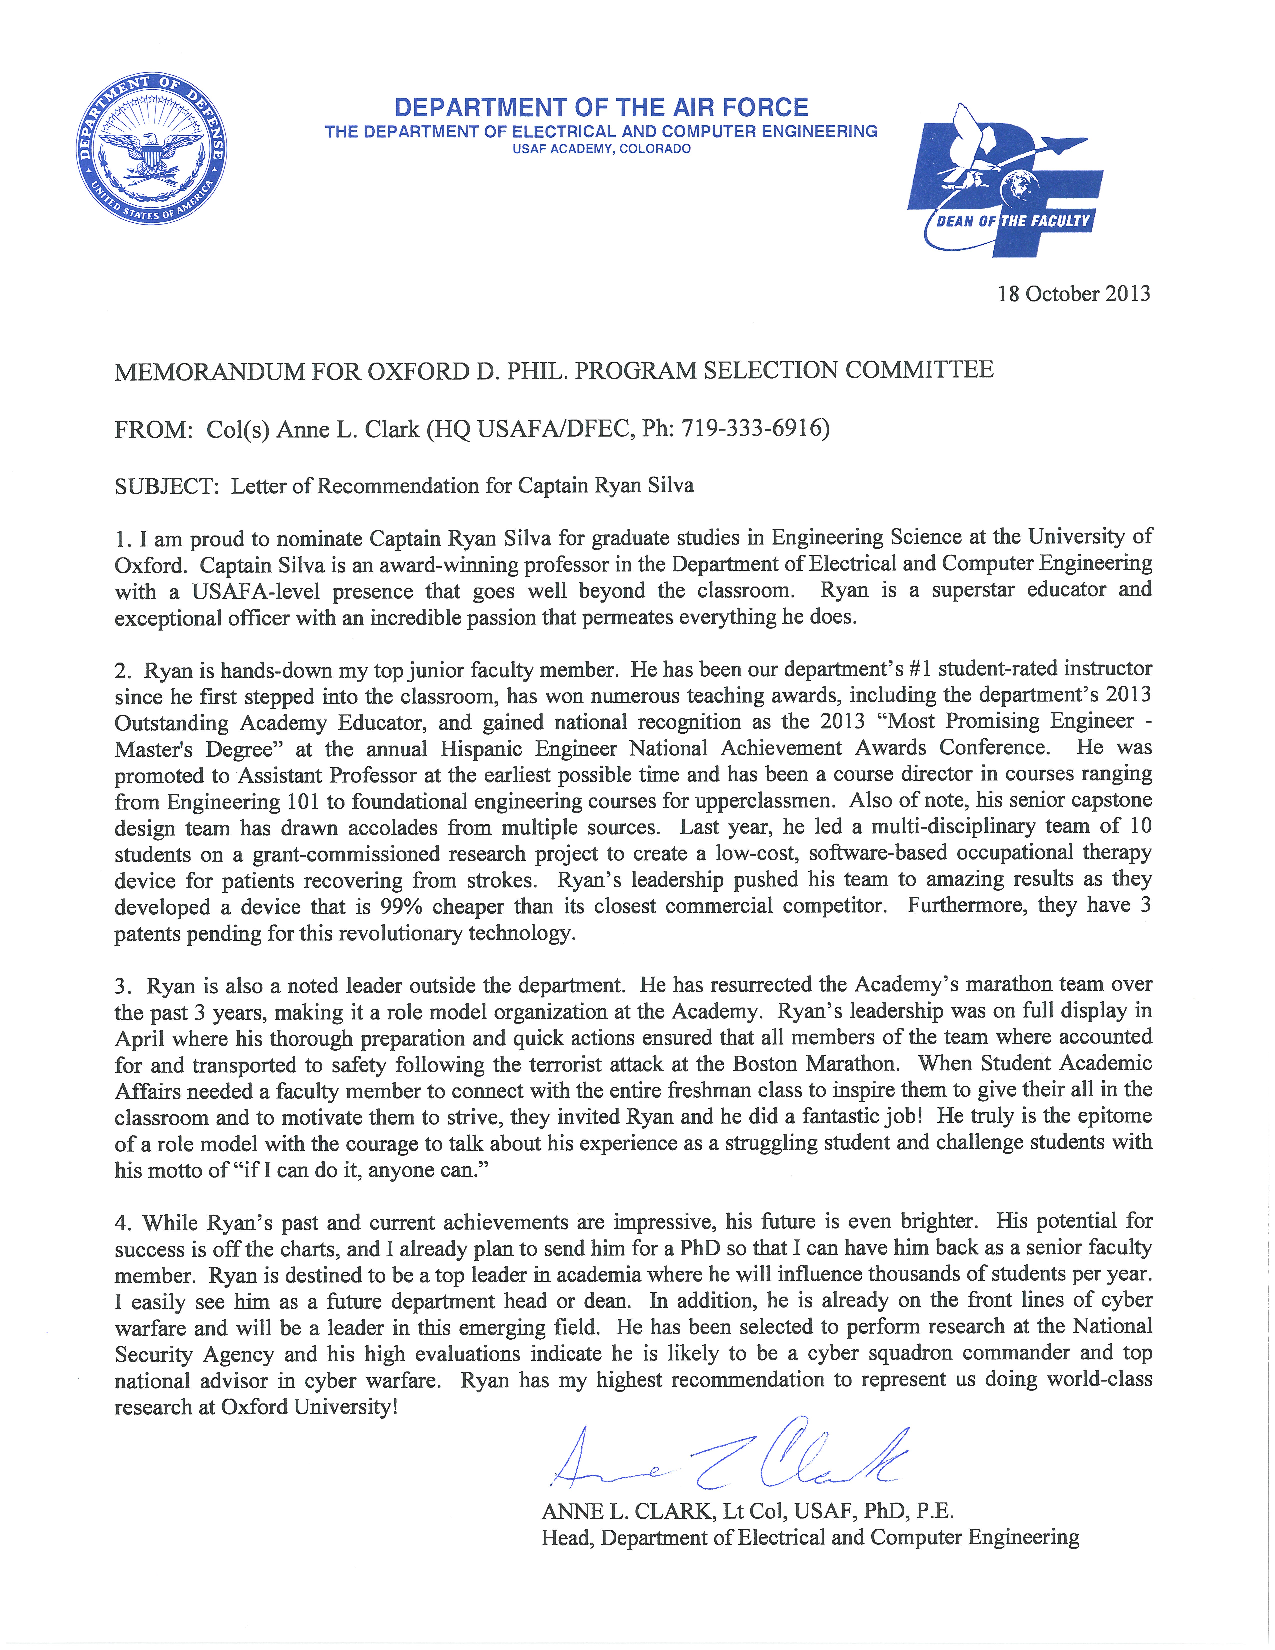
\includegraphics[scale=.85, clip=true, trim=0.5in .5in 1cm 0.4in]{Rec.pdf}

\newpage

\section*{\raggedright Attachment 4 \newline May 2012 - May 2013 OPR}
\addcontentsline{toc}{section}{Attachment 4 - OPR May 2012 - May 2013}
\centering
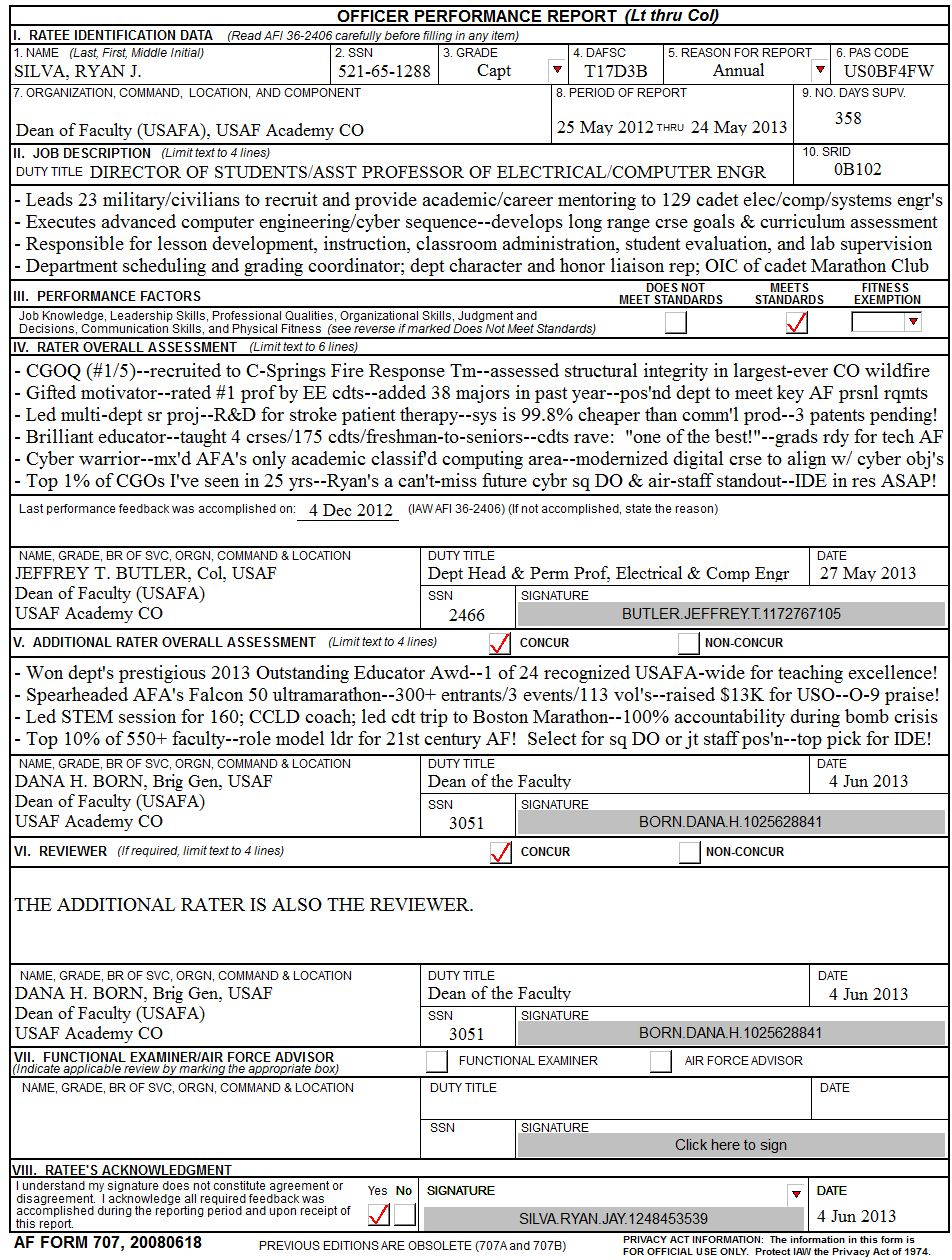
\includegraphics[scale=.63]{OPR2012-2013f}
\newpage
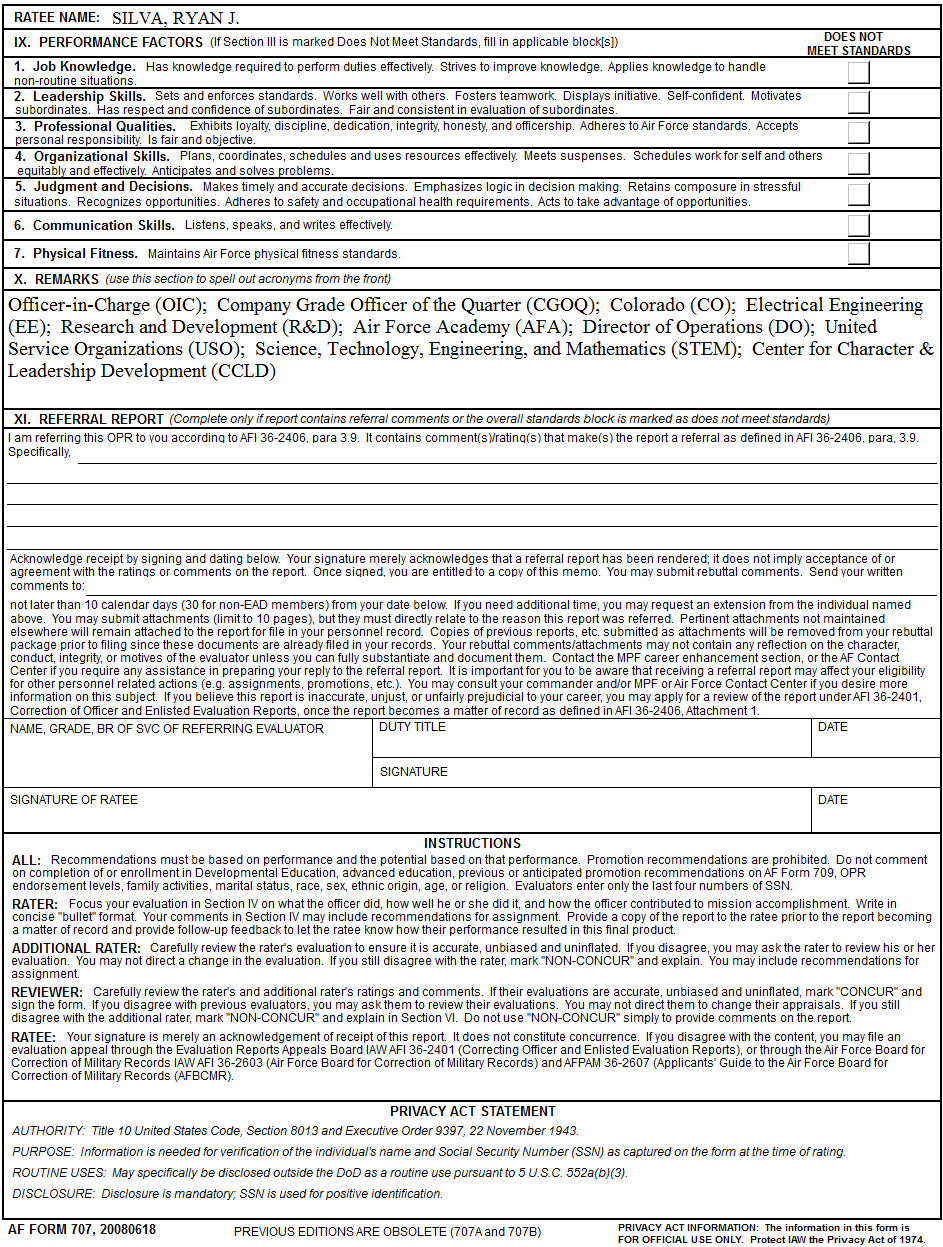
\includegraphics[scale=.65]{OPR2012-2013b}
\label{sec:OPR2012}
\newpage
\section*{\raggedright Attachment 5 \newline May 2011 - May 2012 OPR}
\addcontentsline{toc}{section}{Attachment 5 - OPR May 2011 - May 2012}
\centering
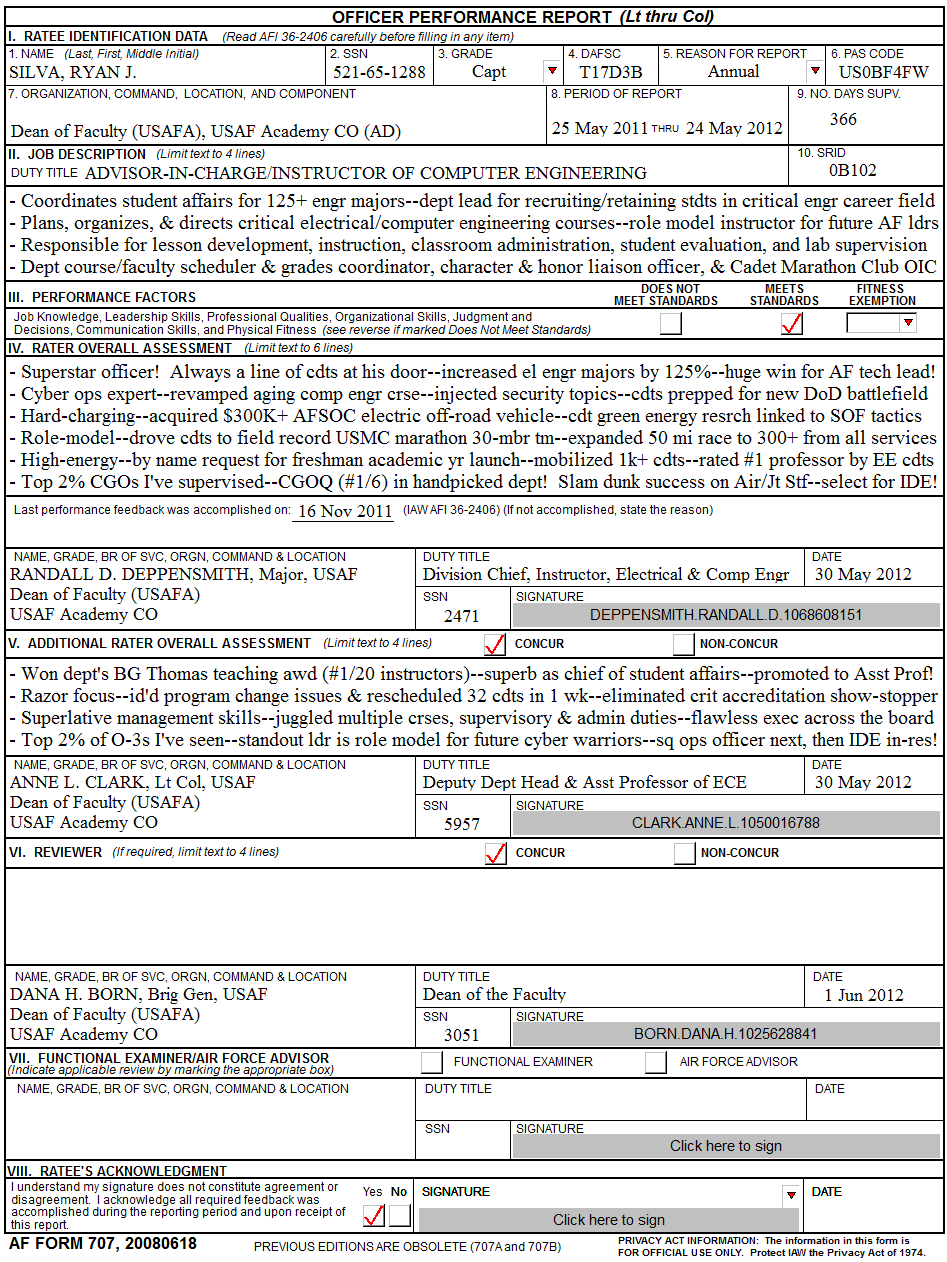
\includegraphics[scale=.63]{OPR2011-2012f}
\newpage
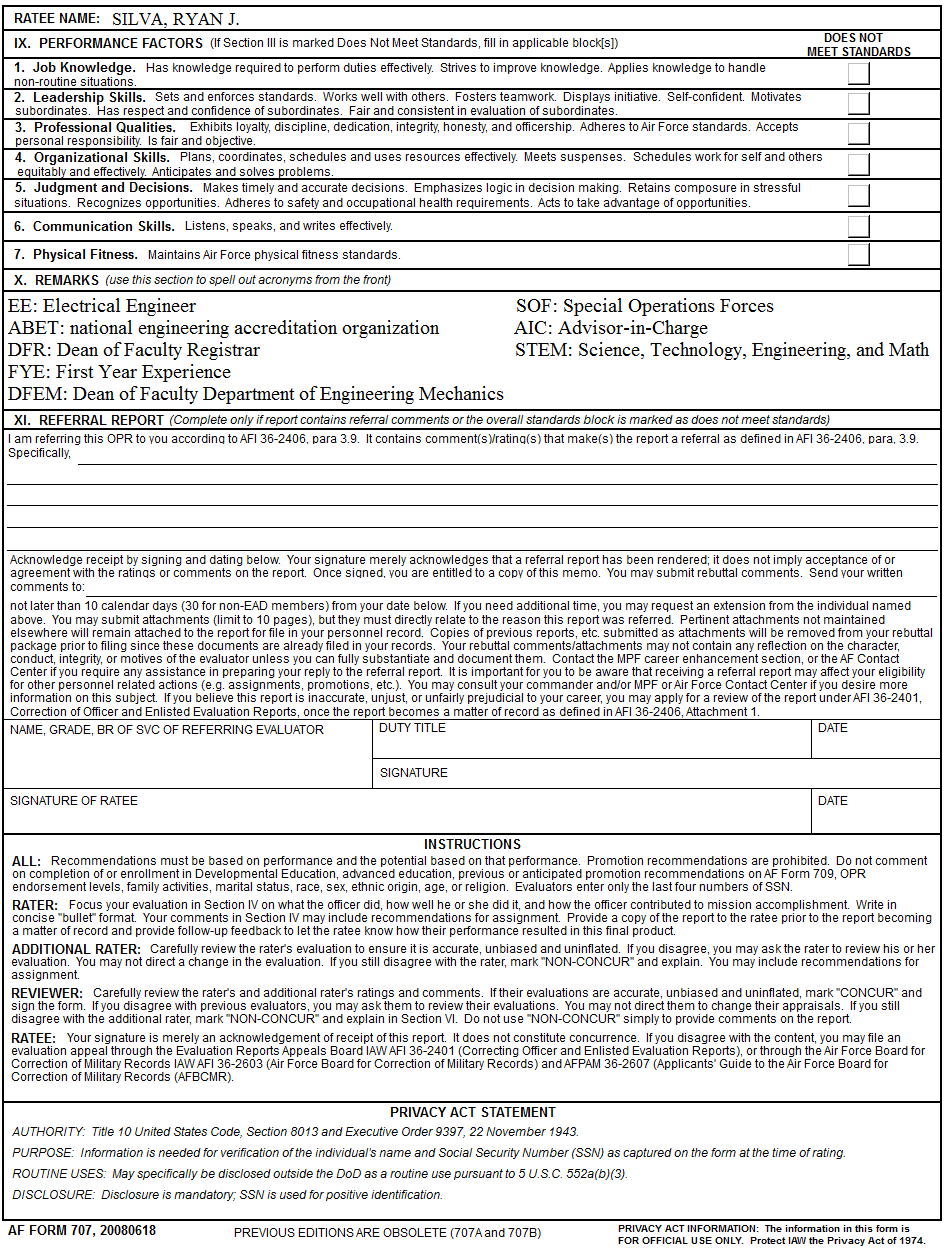
\includegraphics[scale=.65]{OPR2011-2012b}
\section*{\raggedright Attachment 6 \newline May 2010 - May 2011 OPR}
\addcontentsline{toc}{section}{Attachment 6 - OPR May 2010 - May 2011}
\centering
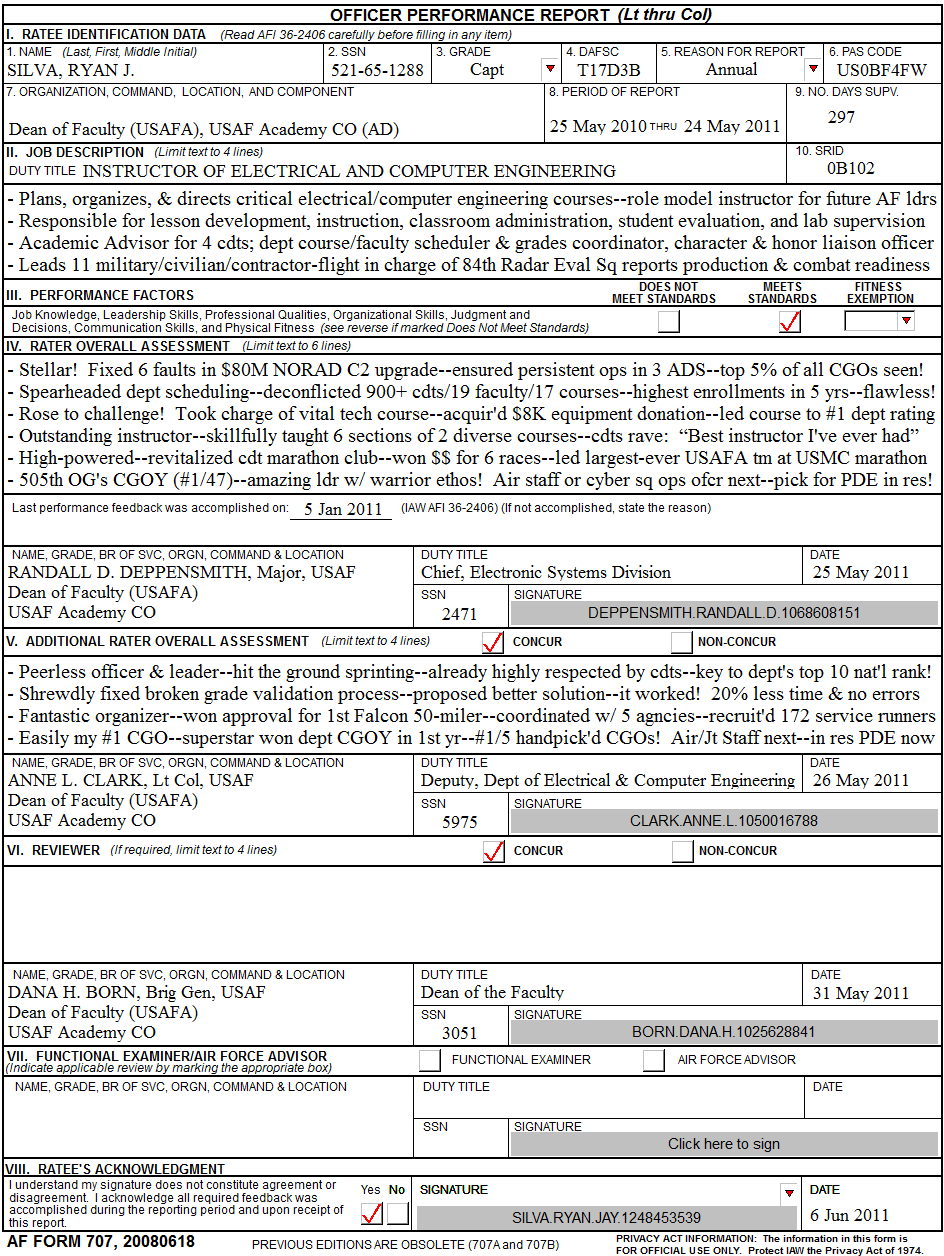
\includegraphics[scale=.63]{OPR2010-2011f}
\newpage
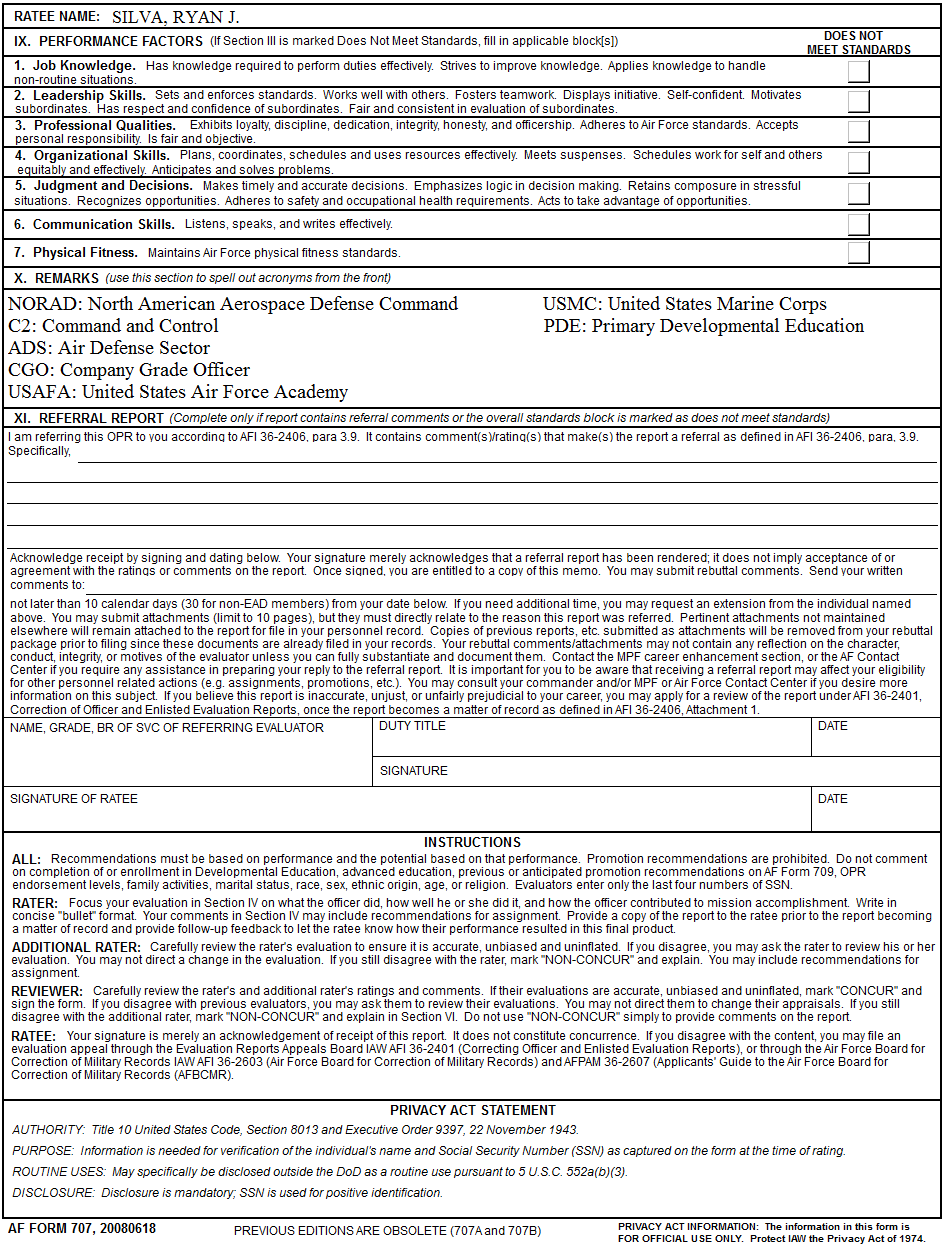
\includegraphics[scale=.65]{OPR2010-2011b}
\section*{\raggedright Attachment 7 \newline Dec 2009 - May 2010 OPR (Change of Rater)}
\addcontentsline{toc}{section}{Attachment 7 - OPR Dec 2009 - May 2010 (CRO)}
\centering
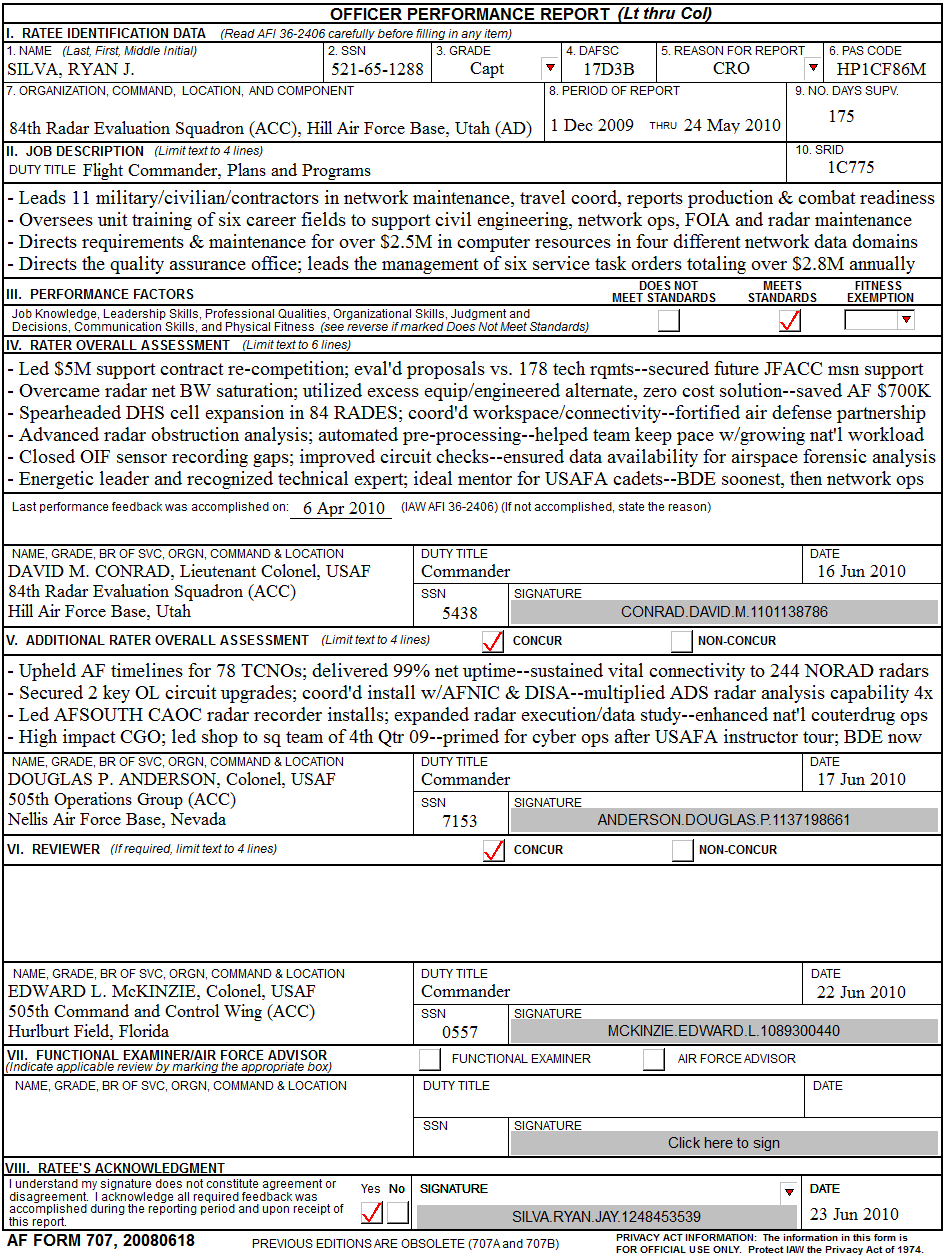
\includegraphics[scale=.63]{OPR2009-2010f}
\newpage
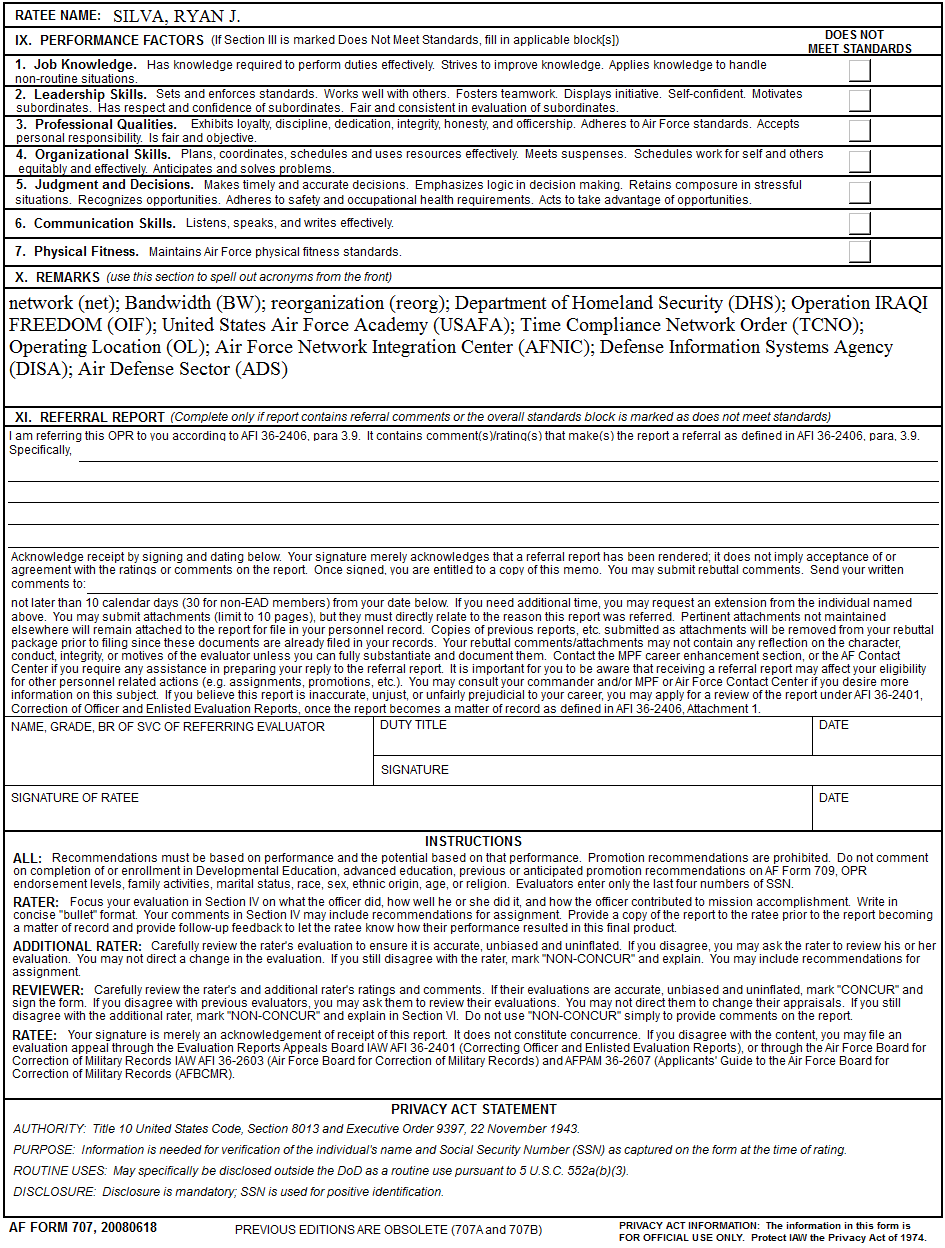
\includegraphics[scale=.65]{OPR2009-2010b}
\section*{\raggedright Attachment 8 \newline Mar 2009 - Nov 2009 OPR (Deployment)}
\addcontentsline{toc}{section}{Attachment 8 - OPR Mar 2009 - Nov 2009 OPR (Deployment)}
\centering
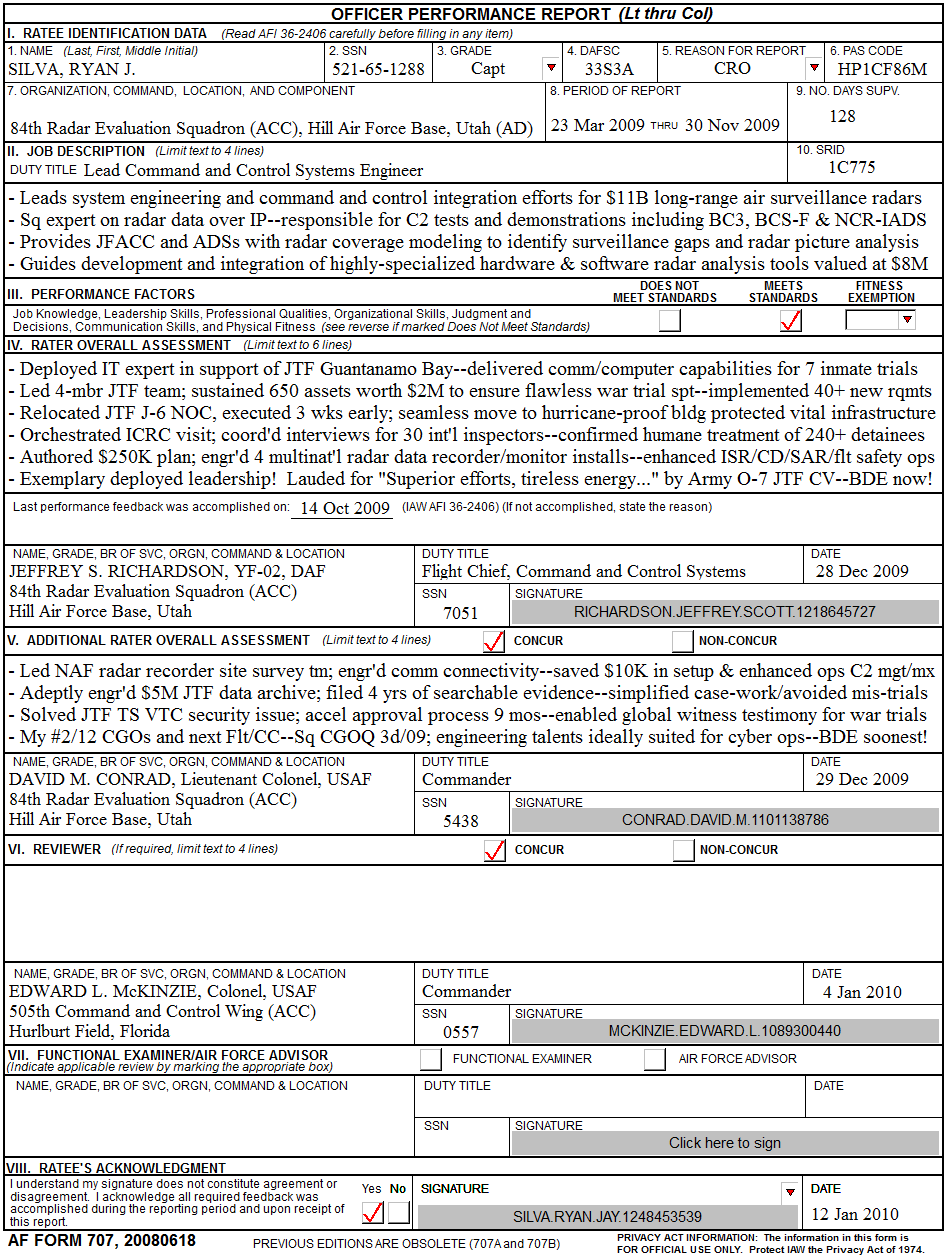
\includegraphics[scale=.63]{DeployOPRf}
\newpage
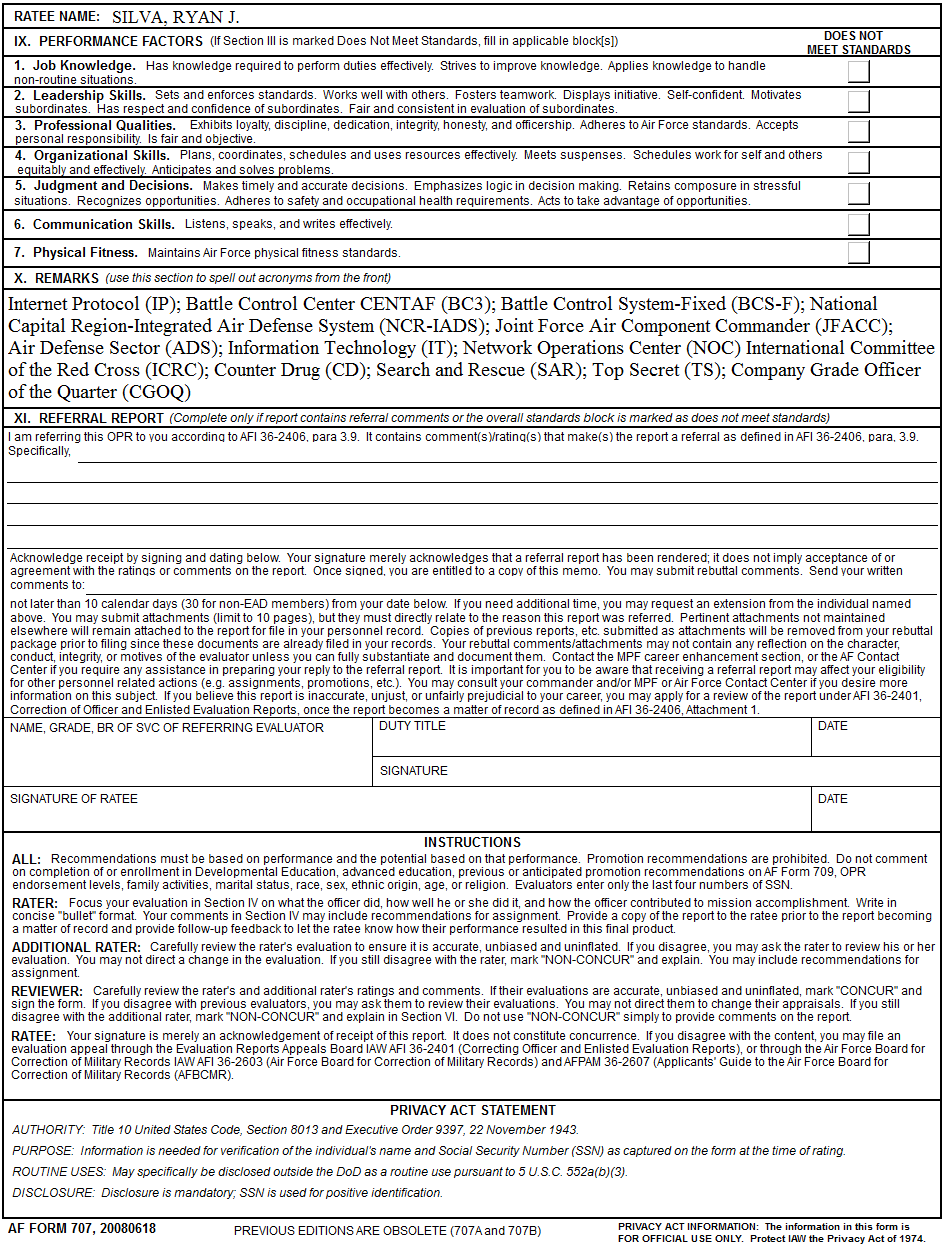
\includegraphics[scale=.65]{DeployOPRb}


%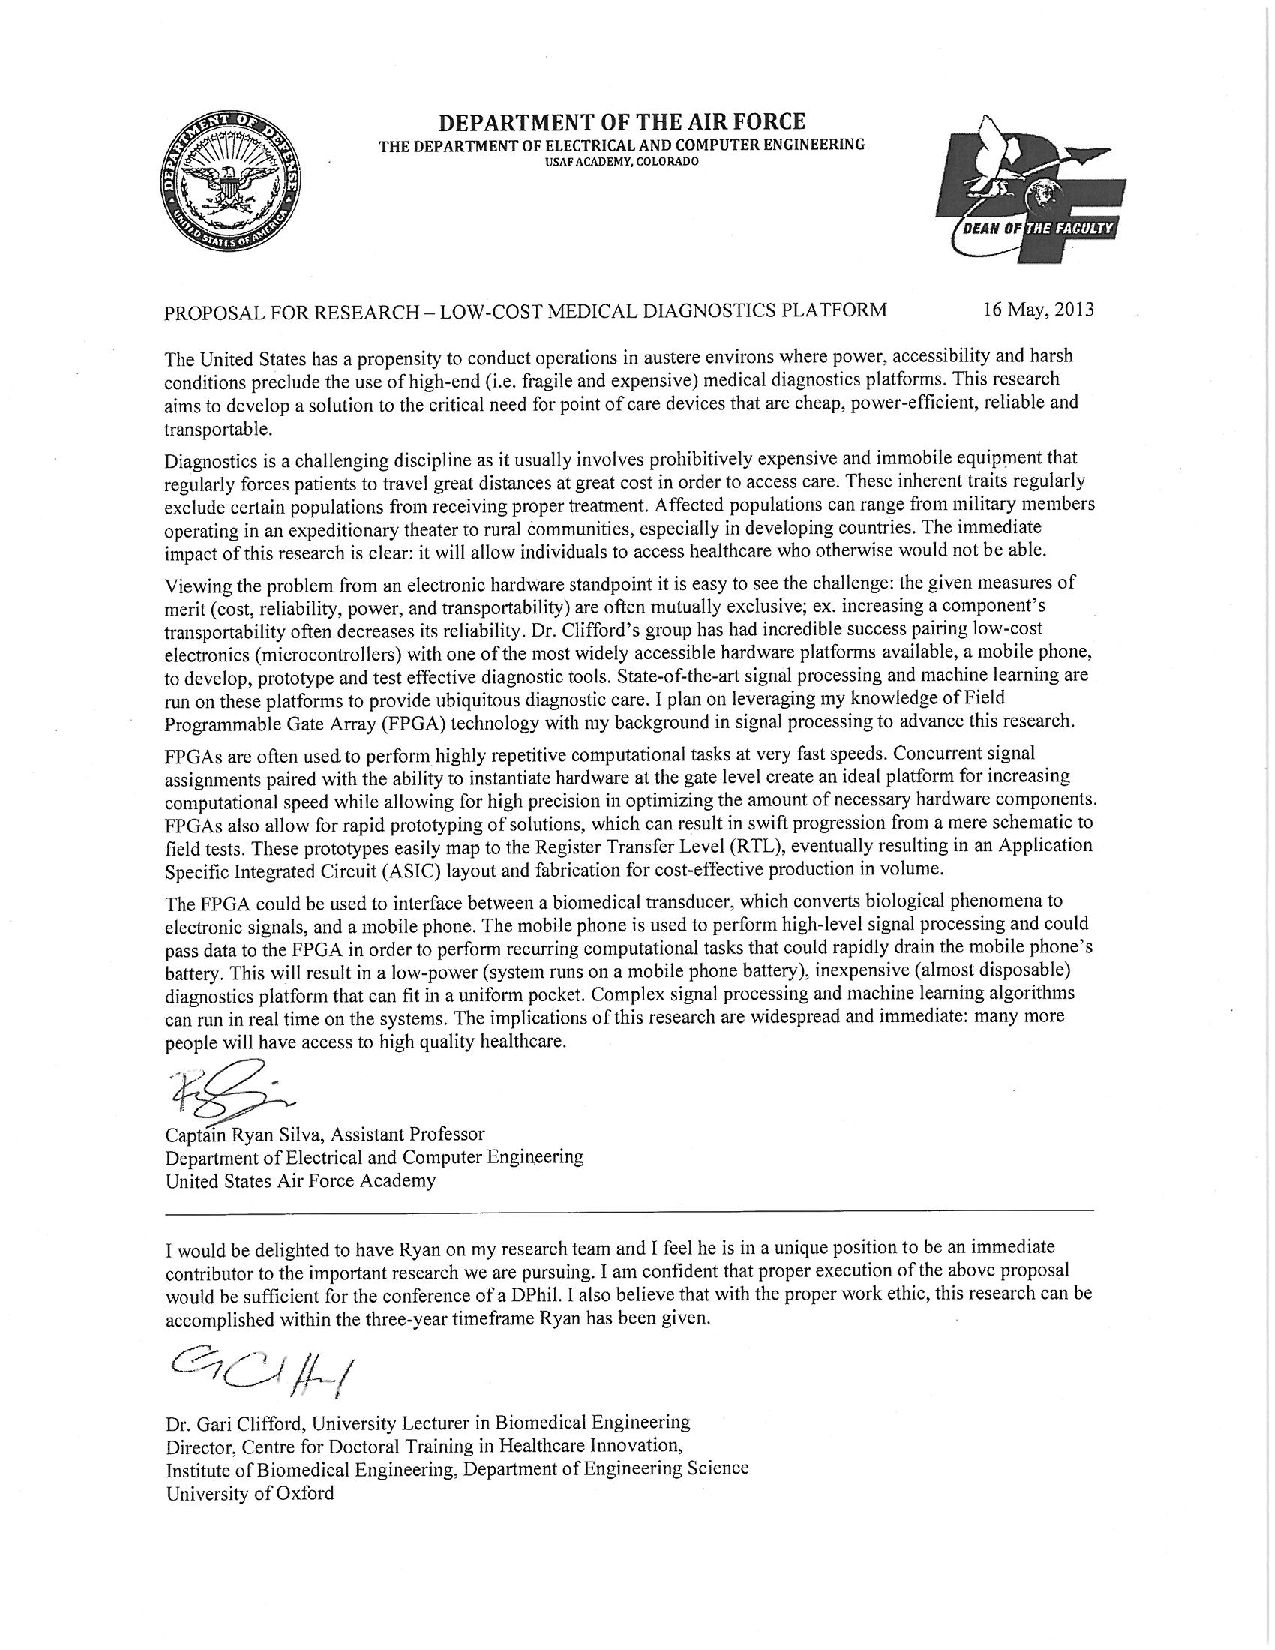
\includepdf[scale=0.8,offset=-25 -25,pagecommand={\section{Attachment - Approved Oxford Research Proposal}\label{sec:prop}}]{MFR_ProposalforResearch_SilvaSIGNED.pdf}

\end{document}
